\vspace{.5cm}
\begin{table}[h]
    \centering
    \begin{tabular}{cc}
        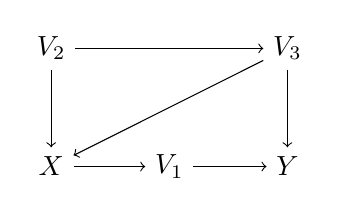
\begin{tikzpicture}
            \node (1) at (0,0) {$X$};
            \node (2) at (3,0) {$Y$};
            \node (3) at (1.5,0) {$V_1$};
            \node (4) at (0,1.5) {$V_2$};
            \node (5) at (3,1.5) {$V_3$};
            \draw[->]  (1) edge (3);
            \draw[->]  (3) edge (2);
            \draw[->]  (4) edge (1);
            \draw[->]  (4) edge (5);
            \draw[->]  (5) edge (1);
            \draw[->]  (5) edge (2);
        \end{tikzpicture}
        \hspace{1cm}
        &
        \hspace{1cm}
        \begin{math}
            \begin{aligned}
                    X&=f_{X}(v_{2}, v_{3}, u_{X}) \\
                    Y&=f_{Y}(v_{1}, v_{3}, u_{Y}) \\
                    V_{1}&=f_{V_{1}}(x, u_{V_{1}}) \\
                    V_{2}&=f_{V_{2}}(u_{V_{2}}) \\
                    V_{3}&=f_{V_{3}}(v_{2}, u_{V_{3}})
            \end{aligned}
        \end{math}
    \end{tabular}
    \caption{Non-parametric SEM with the graphical interpretation of the model.}
    \label{tab:npmodel}
\end{table}
\vspace{.5cm}